\documentclass[12pt]{article}

% Packages
\usepackage{graphicx}
\usepackage{subcaption}
\usepackage{hyperref}

\usepackage[margin=1in]{geometry}

% \usepackage[style=authoryear,maxbibnames=99]{biblatex}
% \addbibresource{tex/publications.bib}
% \DeclareNameAlias{default}{given-family}
\usepackage{natbib}
\bibliographystyle{unsrtnat}
\renewcommand{\bibsection}{}

% No translations, only English
\newcommand{\email}{joel.oskarsson@liu.se}

\graphicspath{{./graphics/}}

\pagenumbering{gobble}
\usepackage[utf8]{inputenc}

\begin{document}

\begin{figure*}
    \begin{subfigure}[]{0.4\textwidth}
        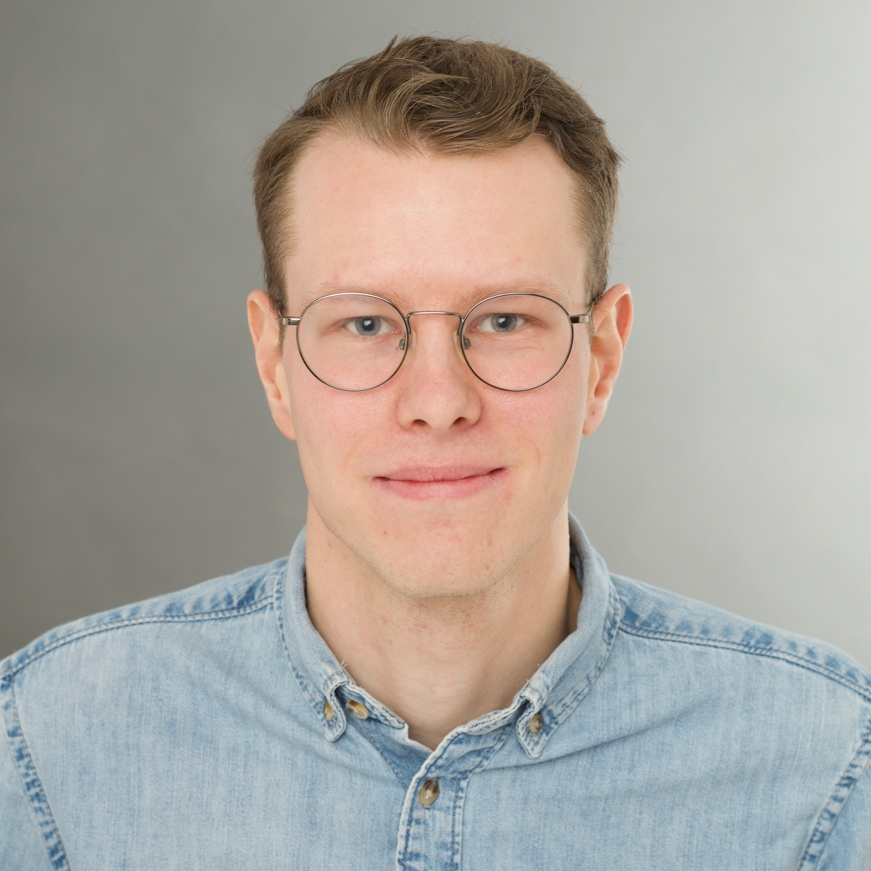
\includegraphics[height=6cm]{photo}
    \end{subfigure}%
    ~
    \begin{subfigure}[]{0.5\textwidth}
        \part*{Joel Oskarsson}

        \begin{tabular}{l l}
            \href{mailto:\email}{\email} & +46706724739\\
            \href{http://joeloskarsson.github.io}{joeloskarsson.github.io} & \href{http://linkedin.com/in/joel-oskarsson}{linkedin.com/in/joel-oskarsson}\\
        \end{tabular}
        \\
        \\

        \begin{tabular}{l l}
            Dept. of Computer and Information Science & \\
            Linköpings universitet & \\
            SE-581 83 Linköping, Sweden & \\
        \end{tabular}

     \end{subfigure}%
\end{figure*}

\section*{Research Interests}
In my research I develop machine learning methods for data with spatial-, temporal- and graph-structure, including combinations of these.
I am interested in how more traditional probabilistic methods in these domains can be combined with deep learning in order to derive new methods with useful properties.
When evaluating and applying these methods to real-world problems I focus on applications within transport and vehicle systems as well as climate and weather modeling.

\section*{Publications}
\nocite{*}
\bibliography{tex/publications.bib}
%\printbibliography[heading=none]

\section*{Education}
\begin{itemize}
    \item In progress: \textbf{Doctoral Studies in Computer Science, Linköping University}, Linköping, Sweden, 240 ECTS\\
        Aug 2020 --
            %In the general area of statistical machine learning. Research focused on machine learning for spatio-temporal problems.
            \begin{itemize}
                \item Part of the Division of Statistics and Machine Learning, Department of Computer and Information Science. Supervised by \href{https://lindsten.netlify.app/}{Fredrik Lindsten} (main supervisor), \href{https://scholar.google.se/citations?user=0UomzRIAAAAJ}{Per Sidén} and \href{https://www.ida.liu.se/~jospe50/}{Jose M. Peña}
                \item PhD project: \textit{Probabilistic Deep Learning for Spatio-Temporal Data Analysis}
                \item Affiliated PhD Student in the \href{https://wasp-sweden.org/}{Wallenberg AI, Autonomous Systems and Software Program}
            \end{itemize}
        \item
            \textbf{Master's program in Computer Science and Engineering (Swedish Civilingenjörsprogram), Linköping University}, Linköping, Sweden, 300 ECTS\\
        Aug 2015 -- June 2020
        \begin{itemize}
            \item Master's thesis: \href{http://urn.kb.se/resolve?urn=urn:nbn:se:liu:diva-166637}{Probabilistic Regression using Conditional Generative Adversarial Networks}
        \end{itemize}

    \item \textbf{Exchange Year, ETH Zürich}, Zürich, Switzerland\\
        Sep 2018 -- Aug 2019\\
            First year of my master's as an exchange student at ETH. Courses mainly in machine learning and AI.
\end{itemize}

\section*{Employment}
\begin{itemize}
    \item \textbf{PhD Student, Linköping University}, Linköping\\
    Aug 2020 --\\
    Apart from my research, I spend 20\% of my employment on teaching. Some notable teaching activities include:
        \begin{itemize}
            \item Co-developing and running the online course \href{https://foundations-of-ml.ida.liu.se/}{\textit{Foundations of Machine Learning}}
            \item Supervising 5 master's thesis projects
            \item Assisting and correcting labs in courses on machine learning, computational statistics and python programming.
        \end{itemize}
    \item \textbf{Teaching Assistant, Linköping University}, Linköping, Sweden\\
        Multiple periods 2016--2019\\
            Held lessons, seminars and lab-sessions for courses in mathematics, computer science and machine learning.
            %Developed my teaching skills and my ability to communicate scientific concepts.
    \item \textbf{Summer Intern, Ericsson}, Linköping, Sweden\\
        Jun-Aug 2018\\
        Internship at Ericsson Research, working with GNSS positioning.

\end{itemize}

\section*{Specific Skills and Knowledge}
\begin{itemize}
    \item Extensive knowledge of models and algorithms for modern \textbf{machine learning and AI} applications. Specific expertise in:
    \begin{itemize}
        \item Graph neural networks
        \item Bayesian models and inference methods
        \item Probabilistic deep learning
    \end{itemize}

\item Sound knowledge of good \textbf{software engineering} practices, acquired from courses and projects throughout my undergraduate studies.
        % I apply these practices to my research projects, creating accessible code.
        % To emphasize transparency and reproducability in research I have made a habit to release research code publicly (see \href{my github page}{https://github.com/joeloskarsson}).

    \item Programming languages and frameworks
    \begin{description}
        \item [Knowledgeable in] Python, PyTorch, PyTorch Geometric and SciPy/NumPy.
        \item [Experience with] R, Tensorflow, scikit-learn, Java, MATLAB and C++.
    \end{description}

\item Highly accustomed to working in \textbf{Linux} environments.
\end{itemize}

% Footer of page 2
\iffalse
\vfill
\center
\begin{tabular}{l l}
    Joel Oskarsson & \href{http://joeloskarsson.github.io}{joeloskarsson.github.io}\\
    \href{mailto:\email}{\email} & +46706724739
\end{tabular}
\fi

\end{document}
